\documentclass[11pt,a4paper]{article}

\usepackage[margin=2.2cm]{geometry}
\usepackage[T1]{fontenc}
\usepackage{lmodern}
\usepackage{amssymb}
\usepackage{xcolor}
\usepackage{tikz}
\usetikzlibrary{arrows.meta,positioning}
\usepackage{booktabs}
\usepackage{tabularx}
\usepackage{enumitem}
\usepackage{listings}
\usepackage[most]{tcolorbox}
\usepackage{fancyhdr}
\usepackage[colorlinks=true,linkcolor=blue!50!black,urlcolor=blue!50!black]{hyperref}

\definecolor{local}{HTML}{2E7D32}
\definecolor{cloud}{HTML}{1565C0}
\definecolor{warn}{HTML}{C62828}
\definecolor{idea}{HTML}{6A1B9A}
\definecolor{soft}{HTML}{F5F5F5}

\newtcolorbox{concept}[1]{colback=idea!4,colframe=idea!70,fonttitle=\bfseries,title={Concept: #1},breakable}
\newtcolorbox{analogy}{colback=local!5,colframe=local!70,fonttitle=\bfseries,title={Analogy},breakable}
\newtcolorbox{why}{colback=cloud!4,colframe=cloud!70,fonttitle=\bfseries,title={Why it is done this way},breakable}
\newtcolorbox{caution}{colback=warn!4,colframe=warn!70,fonttitle=\bfseries,title={Watch out},breakable}
\newtcolorbox{exercise}{colback=soft,colframe=black!50,fonttitle=\bfseries,title={Check yourself},breakable}

\lstset{basicstyle=\ttfamily\small,backgroundcolor=\color{soft},frame=single,
        rulecolor=\color{black!25},columns=fullflexible,keepspaces=true,
        showstringspaces=false,breaklines=true}

\pagestyle{fancy}
\fancyhf{}
\lhead{\small Listen -- Learning Doc 09}
\rhead{\small Errors, Logs, Tests and CI}
\cfoot{\thepage}

\title{\textbf{Listen}\\[4pt]\large Learning Doc 09: Errors, Logs, Tests and CI\\
       \normalsize What happens when things break, and how we know they work}
\author{Detailed design, Section 8}
\date{18 October 2026}

\begin{document}
\maketitle

\begin{abstract}
\noindent Sections 1--7 described Listen when everything goes right. This document covers the
rest: every way a part of the system can fail, what you see and hear when it does, and how
Listen recovers on its own. It then designs the log files, the tests for each part (including
how speech is tested with your own clips without breaking the privacy rule), and continuous
integration with \textbf{GitHub Actions}, explained from scratch, including the many other jobs
it is used for.
\end{abstract}

\tableofcontents
\newpage

% =====================================================================
\section{Decisions this section is built on}
\begin{center}
\renewcommand{\arraystretch}{1.2}
\begin{tabularx}{\textwidth}{l X}
\toprule
\textbf{Topic} & \textbf{Decision} \\
\midrule
Agent crash      & \textbf{Restart automatically}, at most 3 times in 10 minutes, with a pop-up each time; after that, stop and say so. \\
Logs             & \textbf{No spoken words in logs} by default: command ids, timings and errors only. A temporary debug switch adds words. \\
Speech tests     & \textbf{Your own voice}: about 20 clips recorded on purpose, kept \textbf{on your laptop only} (git-ignored, never synced). \\
CI               & \textbf{GitHub Actions} runs every check on every push. \\
From earlier     & Graceful degradation and the thread supervisor (Doc~04); invalid commands are skipped with a warning (Doc~03); sync back-off (Doc~06); one error shape on the server (Doc~07); the four page states (Doc~08). \\
\bottomrule
\end{tabularx}
\end{center}

\begin{caution}
\textbf{The test clips are the one exception to ``no audio is ever saved'' (Doc~05).} The
running assistant still never stores audio. The only recordings are the clips \emph{you} make
deliberately with a developer command, stored in \texttt{agent/tests/audio/clips/}. That folder
is in \texttt{.gitignore}, so your voice never reaches the public GitHub repo, and the sync code
never reads it. A side benefit: the \texttt{tiny.en} vs.\ \texttt{base.en} benchmark can reuse
these clips instead of you speaking every command live each time.
\end{caution}

% =====================================================================
\section{Two kinds of failure}

\begin{concept}{Expected failures vs.\ bugs}
An \textbf{expected failure} is the world not cooperating: the headset is unplugged, the server
is asleep, an app is not installed, you said something Listen has no command for. These are
normal and must be \emph{handled}: tell you clearly, recover, carry on.
A \textbf{bug} is the code being wrong: a typo, a missed case, a crash. Bugs must be
\emph{caught}: contained so the rest keeps working, written to the log with full detail, and
then fixed, with a test so they never return.
\end{concept}

\noindent Three rules follow, and every design choice below applies one of them:
\begin{enumerate}[nosep]
  \item \textbf{Contain.} A failure stays inside the part where it happened. A broken command
        never stops the listener; a broken thread never stops the process (Doc~04's supervisor).
  \item \textbf{Tell, briefly.} You get one clear message in plain words (a chime, a pop-up, a
        web page state), never a wall of technical text. The details go to the log.
  \item \textbf{Recover on its own.} Wherever Listen can retry or reconnect, it does, without
        asking you.
\end{enumerate}

\begin{analogy}
A good restaurant kitchen: if one dish burns, the chef remakes it and the other tables never
notice (contain). The waiter tells that one table ``five more minutes'' rather than describing
the fire (tell briefly). The incident goes in the kitchen log so the cause can be fixed later.
\end{analogy}

% =====================================================================
\section{What can fail, and what happens}

\subsection{On the laptop}
\begin{center}
\small
\renewcommand{\arraystretch}{1.2}
\begin{tabularx}{\textwidth}{>{\raggedright\arraybackslash}p{3.3cm} >{\raggedright\arraybackslash}X >{\raggedright\arraybackslash}X}
\toprule
\textbf{Failure} & \textbf{What you notice} & \textbf{What Listen does} \\
\midrule
No microphone / unplugged & Pop-up ``No microphone found'' & Keeps checking every 2\,s (Doc~04); resumes on its own when one appears. \\
Speech or wake-word model will not load & Pop-up ``Listen can't start: speech model missing'' & Stops at start-up with the exact file named in the log. Nothing can work without it, so pretending would be worse. \\
You said nothing it knows & ``Not caught'' chime (not in continuous mode) & Saved as \emph{no match}; shows in History and Insights' ``sentences that didn't match''. \\
Low confidence & ``Question'' chime / confirm & The two thresholds of Doc~03 decide: run, confirm, or ignore. \\
A command's action fails (app not installed, bad URL) & Pop-up ``Couldn't open Notion'' & Saved as \emph{failed} with the reason; the undo slot is not touched. \\
An action has a bug (raises an error) & Same pop-up & Caught at the action boundary; full traceback to the log; listener carries on. \\
Command file has a mistake after an edit & Pop-up ``core.yaml line 14: unknown slot \{qury\}'' & Invalid entries are skipped, valid ones load (Doc~03). If the whole file cannot be read, the last good version of that file stays in use. \\
A worker thread dies & Nothing, usually & The supervisor restarts it (Doc~04). \\
The whole agent crashes & Pop-up ``Listen restarted after an error'' & Restarted by the launcher, at most 3 times in 10 minutes; then ``Listen stopped, see the log''. Volumes left ducked are restored on start (Doc~04). \\
Database busy & Nothing & Waits up to 5\,s (SQLite's busy timeout) before giving up on that write. \\
Disk full & Pop-up ``Disk full: commands still run but aren't being saved'' & Commands keep working; saving resumes when space is freed. \\
Database file damaged & Pop-up ``History file was damaged; started a new one'' & Checked at start. A damaged file is renamed (kept, not deleted) and a fresh one created. Anything already synced is still on the server. \\
AI builder: no API key or API error & Message in the builder & The builder is disabled without a key; an API error writes nothing to your command files. \\
\bottomrule
\end{tabularx}
\end{center}

\begin{concept}{Launcher (watchdog)}
A process cannot restart itself after it has crashed, because it no longer exists. So Listen is
started by a tiny \textbf{launcher}: a few lines of Python whose only job is to start the agent
as a \emph{child process} and watch it. If the child exits with an error, the launcher counts the
crash and starts it again; after 3 crashes in 10 minutes it stops, because something is
permanently wrong and restarting forever would just hide it. The launcher does no real work, so
it almost never crashes itself, and it costs a few MB of memory.
\end{concept}

\subsection{Between laptop and server}
\begin{center}
\small
\renewcommand{\arraystretch}{1.2}
\begin{tabularx}{\textwidth}{>{\raggedright\arraybackslash}p{3.3cm} >{\raggedright\arraybackslash}X >{\raggedright\arraybackslash}X}
\toprule
\textbf{Failure} & \textbf{What you notice} & \textbf{What Listen does} \\
\midrule
Offline / server asleep / timeout & Nothing; the web app shows ``Last synced 20 min ago'' & Back-off 5/10/20/30 minutes; immediate retry on reconnect (Doc~06). Nothing is lost: the outbox keeps every row. \\
Device token revoked or wrong (401) & Pop-up ``Sync stopped: this laptop's token was revoked. Create a new one in the web app.'' & Stops syncing (retrying would never work) until a new token is in \texttt{agent/.env}. \\
Server rejects a row (422) & Nothing & That row is logged and set aside; the rest of the batch continues. \\
\bottomrule
\end{tabularx}
\end{center}

\subsection{On the server and in the web app}
\begin{itemize}[nosep]
  \item \textbf{One error shape} for every error (Doc~07), now with a \texttt{request\_id}. The
        same id is written in the server log, so ``Error, request 7f3a'' on the web page can be
        found in the log in seconds.
  \item \textbf{Unexpected server errors (500)}: the full traceback goes to the log; the response
        says only ``Something went wrong on the server'', because tracebacks can reveal internals.
  \item \textbf{Database unreachable}: 503 ``Service unavailable''. The laptop treats it like
        being offline and backs off.
  \item \textbf{Web app}: the four states designed in Doc~08 (loading, waking up, error with Try
        again, empty). A 401 sends you to the login page.
\end{itemize}

% =====================================================================
\section{Logs}

\begin{concept}{Log file and log levels}
A \textbf{log} is a text file a program writes as it runs: one line per event, with the time.
When something goes wrong at 2 a.m., the log is how you find out what happened. Each line has a
\textbf{level}, so you can choose how much detail to keep:
\begin{center}
\begin{tabular}{l l}
\texttt{DEBUG}   & Fine detail, only while chasing a problem \\
\texttt{INFO}    & Normal events: started, synced, command ran \\
\texttt{WARNING} & Something odd but handled: invalid command entry, sync retry \\
\texttt{ERROR}   & Something failed: an action raised, a thread died \\
\end{tabular}
\end{center}
The log is set to a level and drops everything below it. Listen runs at \texttt{INFO}.
\end{concept}

\noindent A normal line looks like this, with no spoken words:
\begin{lstlisting}
2026-10-18 14:32:07 INFO  intent   matched core.search conf=0.91 ms_total=1330
2026-10-18 14:32:41 WARN  commands core.yaml:14 skipped: unknown slot {qury}
2026-10-18 14:35:00 INFO  sync     uploaded 12 rows, cursor=4821
\end{lstlisting}

\begin{itemize}[nosep]
  \item \textbf{Where}: \texttt{agent/logs/listen.log} (git-ignored).
  \item \textbf{Rotation}: when the file reaches 1\,MB it is renamed \texttt{listen.log.1} and a
        new one starts; only 5 old files are kept. The logs can never grow past about 5\,MB, so
        they never ``flood'' your disk.
  \item \textbf{No words by default.} What you said is already in the database, where you can
        see and delete it. A copy in a forgotten text file is the kind of thing that gets shared
        by accident. For debugging, \texttt{listen debug on} adds words to the log until the
        next restart, so it can never be left on forever.
  \item \textbf{Server}: logs go to standard output, which the free host collects and shows in its
        dashboard. Same rule: no transcripts, no passwords, no tokens.
\end{itemize}

\begin{why}
A privacy rule that depends on someone remembering it eventually fails. So, as with sync
(Doc~06), a test checks it: run a fake command through the agent with logging captured, and
fail if the heard sentence appears anywhere in the log output.
\end{why}

% =====================================================================
\section{Testing}

\subsection{The test pyramid}
\begin{center}
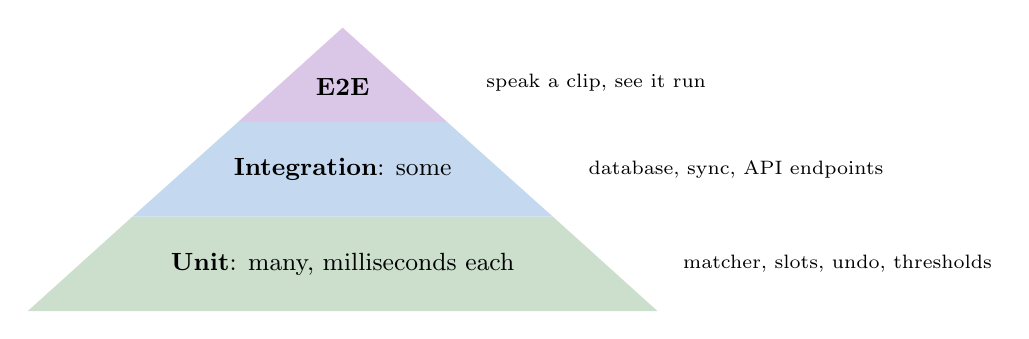
\begin{tikzpicture}
  \fill[local!25] (-4,0) -- (4,0) -- (2.67,1.2) -- (-2.67,1.2) -- cycle;
  \fill[cloud!25] (-2.67,1.2) -- (2.67,1.2) -- (1.33,2.4) -- (-1.33,2.4) -- cycle;
  \fill[idea!25]  (-1.33,2.4) -- (1.33,2.4) -- (0,3.6) -- cycle;
  \node at (0,0.6)  {\small\textbf{Unit}: many, milliseconds each};
  \node at (0,1.8)  {\small\textbf{Integration}: some};
  \node at (0,2.85) {\small\textbf{E2E}};
  \node[anchor=west,font=\scriptsize] at (4.2,0.6) {matcher, slots, undo, thresholds};
  \node[anchor=west,font=\scriptsize] at (3,1.8)   {database, sync, API endpoints};
  \node[anchor=west,font=\scriptsize] at (1.7,2.9) {speak a clip, see it run};
\end{tikzpicture}
\end{center}

\begin{concept}{Unit, integration, end-to-end}
A \textbf{unit test} checks one small piece alone (``does the matcher pull
\texttt{what is an atom} out of \texttt{search what is an atom}?''). It is fast and points at the
exact broken line. An \textbf{integration test} checks pieces working together (``a command saved
by the agent is uploaded by sync and appears on the server''). An \textbf{end-to-end (E2E)} test
runs the whole chain like a user would. E2E tests catch the most but are slow and, when they
fail, do not say where. So: many unit tests, some integration tests, very few E2E tests.
\end{concept}

\subsection{What gets tested, part by part}
\begin{center}
\small
\renewcommand{\arraystretch}{1.2}
\begin{tabularx}{\textwidth}{>{\raggedright\arraybackslash}p{2.6cm} >{\raggedright\arraybackslash}X >{\raggedright\arraybackslash}p{2.4cm}}
\toprule
\textbf{Part} & \textbf{Tests} & \textbf{Where they run} \\
\midrule
Matcher, slots, thresholds & Table of sentences $\to$ expected command and slots, including near-misses and regressions (Doc~03) & Everywhere \\
Command files & Every file in \texttt{commands/} is valid and its example sentences match & Everywhere \\
Undo, routines, continuous-mode guardrails & Sequences of fake commands with a fake clock (``61 s later, undo says can't'') & Everywhere \\
Actions & Run against \textbf{fakes} that record what would have happened, so tests never open apps or change your volume & Everywhere \\
Database & Real SQLite in a temporary file: migrations, WAL, 30-day purge, damaged-file recovery & Everywhere \\
Sync client & Against a fake server: back-off, 401 stop, batches, tombstones, the privacy test & Everywhere \\
Logs & The no-words test above & Everywhere \\
Speech & Your clips $\to$ both models $\to$ check the words and the time against the 500\,ms budget & \textbf{Your laptop only} \\
Server & Every endpoint: happy path, 401, 422; sync edge cases; fresh PostgreSQL per run (Doc~07) & Everywhere \\
Web app & Type check; component tests with a mocked API (Doc~08); the generated API types are up to date & Everywhere \\
\bottomrule
\end{tabularx}
\end{center}

\begin{concept}{Test doubles: fakes and mocks}
Real actions have side effects: launching CLion in a test would be slow and annoying, and
changing your volume during a test run would be worse. So tests swap the real thing for a
\textbf{test double}. A \textbf{fake} is a small working stand-in, for example
\texttt{FakeActions}, which just appends \texttt{("launch\_app", "clion")} to a list the test then
checks. A \textbf{mock} is a stand-in that records calls automatically (Python's
\texttt{unittest.mock}). This is possible because of the design in Doc~03: the matcher decides
\emph{what} to do, and only the action layer touches Windows.
\end{concept}

\paragraph{Speech tests with your clips.} The developer command \texttt{listen record-tests}
reads each test sentence on screen (``search what is an atom'', ``open vs code'' \ldots), records
you saying it, and saves it as \texttt{agent/tests/audio/clips/<id>.wav} with the expected text.
The speech tests then:
\begin{lstlisting}
@pytest.mark.skipif(not CLIPS.exists(), reason="no local clips")
def test_base_en_hears_search(clip="search_atom"):
    text, ms = transcribe(load(clip), model="base.en")
    assert text == "search what is an atom"
    assert ms < 500          # the speech-to-text budget (Doc 04)
\end{lstlisting}
\noindent \texttt{skipif} means: on a machine without the clips (GitHub's), the test is reported
as \emph{skipped}, not failed.

\subsection{Writing tests first}
\begin{concept}{Test-driven development (TDD)}
\textbf{TDD} means writing the test \emph{before} the code, in a three-step loop:
\textbf{red} (write a test for the next small behaviour; run it; it fails, because the code does
not exist yet), \textbf{green} (write the simplest code that makes it pass), \textbf{refactor}
(tidy the code; the test proves you did not break it). The red step matters: a test you have
never seen fail might not be testing anything. Listen is built this way, one small behaviour at a
time; the implementation plan after this design is written as a list of these loops.
\end{concept}

% =====================================================================
\section{GitHub Actions}

\subsection{What it is}
\begin{concept}{Continuous integration (CI)}
\textbf{Continuous integration} means every change is automatically checked as soon as it is
pushed: the code is installed on a clean machine and every test and check runs. If something
fails, you find out minutes after the change, while you still remember what you did, instead of
weeks later.
\end{concept}

\noindent \textbf{GitHub Actions} is GitHub's built-in automation service. You put a
\textbf{workflow} file (YAML, like our command files) in \texttt{.github/workflows/} in the repo.
It says \emph{when} to run (for example, on every push) and \emph{what} to run. GitHub then starts
a fresh virtual machine, called a \textbf{runner}, copies your repo onto it, follows the steps,
and throws the machine away. The result appears next to the commit as a green \checkmark{} or a
red \texttimes.

\begin{center}
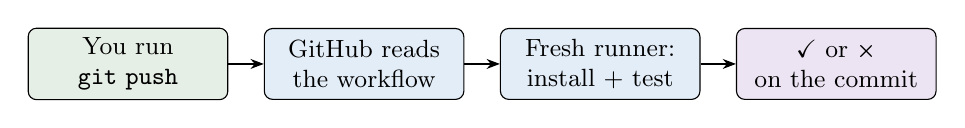
\begin{tikzpicture}[node distance=0.45cm,
  b/.style={draw,rounded corners=3pt,align=center,font=\small,minimum height=0.9cm,text width=2.3cm}]
  \node[b,fill=local!12] (push) {You run\\\texttt{git push}};
  \node[b,fill=cloud!12,right=of push] (gh) {GitHub reads\\the workflow};
  \node[b,fill=cloud!12,right=of gh] (run) {Fresh runner:\\install + test};
  \node[b,fill=idea!12,right=of run] (res) {\checkmark{} or \texttimes{}\\on the commit};
  \draw[-{Stealth}] (push) -- (gh);
  \draw[-{Stealth}] (gh) -- (run);
  \draw[-{Stealth}] (run) -- (res);
\end{tikzpicture}
\end{center}

\subsection{The vocabulary}
\begin{center}
\renewcommand{\arraystretch}{1.15}
\begin{tabularx}{\textwidth}{l X}
\toprule
\textbf{Word} & \textbf{Meaning} \\
\midrule
Workflow & One YAML file describing an automation. A repo can have many. \\
Trigger (\texttt{on:}) & The event that starts it: a push, a pull request, a schedule, a button click. \\
Job & A group of steps that runs on one runner. Jobs run in parallel unless told to wait. \\
Runner & The virtual machine: Ubuntu, Windows or macOS, fresh for every run. \\
Step & One command (\texttt{run: pytest}) or one ready-made action. \\
Action (\texttt{uses:}) & A reusable step someone published, e.g.\ \texttt{actions/checkout} copies your repo onto the runner. \\
Service container & An extra program the job needs, e.g.\ a PostgreSQL database for the server tests. \\
Secret & An encrypted value (API key, deploy token) the workflow can use but never prints. \\
\bottomrule
\end{tabularx}
\end{center}

\subsection{Listen's workflow}
One workflow, \texttt{.github/workflows/ci.yml}, three jobs running side by side:
\begin{lstlisting}
name: CI
on: [push, pull_request]            # trigger: every push and pull request

jobs:
  agent:
    runs-on: windows-latest         # the agent uses Windows-only libraries
    steps:
      - uses: actions/checkout@v4   # copy the repo onto the runner
      - uses: actions/setup-python@v5
        with: { python-version: "3.11" }
      - run: pip install -e "agent[dev]"
      - run: ruff check agent       # style and common mistakes
      - run: pytest agent           # speech tests skip: no clips here

  server:
    runs-on: ubuntu-latest
    services:
      postgres:                     # a throwaway database for the tests
        image: postgres:16
        env: { POSTGRES_PASSWORD: test }
        ports: ["5432:5432"]
    steps:
      - uses: actions/checkout@v4
      - uses: actions/setup-python@v5
        with: { python-version: "3.11" }
      - run: pip install -e "server[dev]"
      - run: pytest server

  web:
    runs-on: ubuntu-latest
    steps:
      - uses: actions/checkout@v4
      - uses: actions/setup-node@v4
        with: { node-version: "20" }
      - run: npm ci --prefix web
      - run: npm run check --prefix web   # type check, tests, API types up to date
\end{lstlisting}

\begin{why}
\textbf{Clean machine:} ``it works on my laptop'' often means it only works because of something
installed long ago. The runner has nothing, so a missing dependency fails here instead of on
deploy day. \textbf{Every push:} the smaller the change being checked, the easier it is to see
what broke. \textbf{Three jobs:} the agent needs Windows, the server needs PostgreSQL; separate
jobs give each exactly what it needs and run in parallel, so the whole check takes a few minutes.
\end{why}

\paragraph{How it helps day to day.}
\begin{itemize}[nosep]
  \item You push, carry on working, and get a red \texttimes{} (with the failing test's output) if
        something broke. Nothing to remember to run.
  \item Later, \textbf{branch protection} can require the check to be green before anything is
        merged into \texttt{main}, so \texttt{main} always works.
  \item A \textbf{status badge} in the README shows visitors that the project's tests pass.
\end{itemize}

\paragraph{Cost.} Free and unlimited for public repositories like Listen. Private repositories
get a free monthly allowance (2{,}000 minutes at the time of writing); Windows runners use it up
twice as fast as Linux ones.

\subsection{Other things GitHub Actions is used for}
CI is the most common use, but a workflow can run \emph{anything} on any trigger:
\begin{center}
\small
\renewcommand{\arraystretch}{1.2}
\begin{tabularx}{\textwidth}{>{\raggedright\arraybackslash}p{3.4cm} X}
\toprule
\textbf{Use} & \textbf{What it does} \\
\midrule
Continuous deployment (CD) & After the checks pass on \texttt{main}, deploy automatically: upload the server to the host, publish the web app. Listen will use this in the deployment phase. \\
Releases & On a version tag (\texttt{v1.0}), build the agent into a Windows installer or \texttt{.exe} and attach it to a GitHub Release. \\
Scheduled jobs & \texttt{on: schedule} with a cron time, e.g.\ every Monday check dependencies for known security holes. \\
Dependency updates & Dependabot opens pull requests when a library has a new version; CI tests them before you merge. \\
Security scanning & CodeQL reads the code looking for vulnerabilities; secret scanning blocks pushed API keys. \\
Publishing & Push a Python package to PyPI or a JavaScript package to npm on release. \\
Docs and sites & Build documentation (even LaTeX PDFs like these) and publish it to GitHub Pages. \\
Repo housekeeping & Label new issues, welcome first-time contributors, close stale issues. \\
Anything else & Nightly data jobs, posting to Slack or Discord when a build fails, checking links. \\
\bottomrule
\end{tabularx}
\end{center}

\begin{caution}
Workflows run code with access to the repo's \textbf{secrets}. Keep secrets out of the workflow
file itself (use the repo's encrypted Secrets settings), use well-known actions pinned to a
version, and remember that pull requests from other people's forks do not get your secrets, by
design. Listen's CI needs no secrets at all: the tests use fakes and a throwaway database.
\end{caution}

% =====================================================================
\section{Glossary}
\begin{description}[style=nextline,leftmargin=1.2cm,itemsep=2pt]
  \item[CI / CD] Automatically checking / deploying every change.
  \item[E2E test] A test that runs the whole system the way a user would.
  \item[Expected failure] The world not cooperating (offline, unplugged); handled, not a bug.
  \item[Fake / mock] Test stand-ins for real parts; a fake works simply, a mock records calls.
  \item[GitHub Actions] GitHub's service that runs workflows on events such as a push.
  \item[Integration test] A test of several parts working together.
  \item[Launcher (watchdog)] A tiny process that starts the agent and restarts it after a crash.
  \item[Log level] DEBUG, INFO, WARNING, ERROR: how important a log line is.
  \item[Log rotation] Starting a new log file at a size limit and keeping only a few old ones.
  \item[Request id] A short id on each server request, shown with an error and written in the log.
  \item[Runner] The fresh virtual machine a GitHub Actions job runs on.
  \item[TDD] Test-driven development: red, green, refactor.
  \item[Unit test] A test of one small piece on its own.
  \item[Workflow / job / step] A CI file / a group of steps on one runner / one command.
\end{description}

% =====================================================================
\section{Check your understanding}
\begin{exercise}
\begin{enumerate}
  \item Your headset is unplugged mid-sentence. Which part notices, what do you see, and what
        happens when you plug it back in?
  \item Why does the launcher stop after 3 crashes in 10 minutes instead of restarting forever?
  \item Why does a revoked token stop syncing completely, while ``server asleep'' only backs off?
  \item You add a test and it passes the first time you run it, before you wrote any code. What
        should worry you?
  \item Your speech tests pass on your laptop but show as \emph{skipped} on GitHub. Is that a
        problem? Why are they skipped?
  \item The agent tests run on \texttt{windows-latest} but the server tests on
        \texttt{ubuntu-latest}. Why not the same for both?
  \item Name two things other than running tests that Listen could use GitHub Actions for later.
\end{enumerate}
\end{exercise}

\end{document}
